\chapter{Molecular Dynamics}

Statistical mechanics is fundamentally based upon using the microscopic properties of a system to predict and explain its macroscopic behaviour.\cite{StatMech}
Such studies usually involve sampling the phase space of a system in order to calculate averages of micrscopic properties that relate to a macroscopic observables.
The phase space, however, is obtrusively large and it is simply not practical to conduct a full ensemble average; one must instead be content with a representative sample.\cite{Bopp2008}
Practically this is carried out with computational simulations which either directly sample phase--space trajectories (Molecular Dynamics) or which sample configurational space (Monte-Carlo).
The Marangoni flow is inherentely a dynamic phenomenon and must be studied using a dynamic method, in this case Molecular Dynamics (henceforth MD).

\section{The Lennard--Jones Fluid}
The basic strategy of MD is to sample a system by solving Newton's equations of motions.
This is achieved by calculating the forces acting on each particle at a given time, $t$, and then integrating the equations of motion to infer the position and velocity at time $t + \delta t$.
In order to maintain conservation of energy and satisfy detailed balance, the Verlet algorithm is used to give
\begin{align}
\label{VerletPos}
\mathbf{r}( t + \delta t) &= 2 \mathbf{r}(t) - \mathbf{r}(t-\delta t) + \frac{\mathbf{f}(t)}{m} \delta t ^ {2}\\
\label{VerletVel}
\mathbf{v}(t) &= \frac{\mathbf{r}(t+\delta t) - \mathbf{r}(t-\delta t)}{2 \delta t},
\end{align}
where Eqn. \ref{VerletPos} has the distinct advantage of being symmetric with respect to time--inversion.

To simplify the subsequent simulation, the fluid was modelled using spherical Lennard--Jones particles with the pair--wise potential:
\begin{equation}
V \left( \mathbf{r}^{\mathrm{N}} \right) = \frac{1}{2} \sum_{i\neq j} \phi \left( r_{ij} \right)
\end{equation}
where
\begin{equation}
\label{LJ}
\phi \left( r_{ij} \right) = 4 \epsilon \left( \left( \frac{\sigma}{r}\right)^{12} - \left( \frac{\sigma}{r}\right)^{6} \right).
\end{equation}
The parameter $\sigma$ controls the length--scale of the potential and is used as the unit of length in the simulations.
To reduce the computational cost of calculating the pair--wise sum, only the contribution from pairs of particles within $4\sigma$ of each other is included.
$\epsilon$ gives the strength of the interaction and the relative values for two different types of particles can be used to control the miscibility of two fluids, as shown in Fig. \ref{Miscibility}.

\section{An isothermal--isobaric ensemble}
Controlling the temperature and pressure of a fluid is essential if the properties of that fluid are to be investigated.
This is done using thermostats and barostats which simulate coupling of the system to an external heat bath or volume.

Thermostats commonly work by applying a stochastic frictional force to particles, either by adding a random force to momenta (Langevin)\cite{Langevin} or reassinging the velocity of a randomly chosen particle from the Maxwell distribtuion (Anderson)\cite{AndersonTherm}.
In this study, the Nos\'{e}--Hoover thermostat is used,  adding an extra term into the equations of motion to provide the effect of an external heat bath.\cite{NoseHoover1, NoseHoover2, NoseHoover3}
The result is that the energy of the simulated system fluctuates whilst the total energy of the system and heat bath remains constant, thus maintaining a canonical ensemble.

The bulk pressure of the fluid must be held constant for all simulations, since if this were not true then body forces could occur in the fluid bulk.
A piston is the simplest way to control the bulk pressure and is relatively easy to create; the fluid is confined between two solid walls and a force equal to $\frac{P_{ext}}{A_{wall}}$ is applied.
In the case of studying Marangoni flows this does, however, come with the limitation that a Marangoni effect will occur at the liquid--solid boundary \textit{as well} as the liquid--liquid interface.
Despite this, if the solid--liquid Marangoni force can be ignored and non--slip wall boundary conditions exist, then a piston comes with the advantage of holding the bulk fluid at rest.

Alternatively a Nos\'{e}--Hoover barostat can employed to control the pressure by altering the box dimensions and ajusting the equations of motion. \cite{NoseHoover1, NoseHoover2, NoseHoover3}
It is important to note that the box dimensions must only be allowed to change in the direction normal to the interface, since any other change will alter the area of the interface and strongly affect the thermodynamic pressure
\begin{equation}
P = - \left( \frac{\partial F}{\partial V} \right)_{T} + \gamma \left( \frac{\partial A}{\partial V} \right)_{T}.
\end{equation}

\section{Estimating statistical error}
With all experiments it is important to have a method of quantifying the statistical error in data, and computer simulations are not exempt.
The measurements made in a molecular dynamics simulation are time-averages of observable and are evaluated over some finite simulation time as
$$A_{\tau} = \frac{1}{\tau} \int_{t=0}^{\tau} A(t) dt.$$
Frenkel and Smit show us that the variance in this average may be calculated as 
$$\sigma^{2}(A) = \frac{1}{\tau^{2}} \int_{0}^{\tau} \int_{0}^{\tau} dt dt' \big \langle [ A(t) - \langle A \rangle ] [A(t') - \langle A \rangle] \big \rangle$$
where the integrand is simply the time-correlation function of fluctations in A\cite{FrenkelSmit}.
In the limit of a simulation time longer than the characteristic decay time $t_{A}^c$ of the correlation function, this error reduces to 
$$\sigma^{2}(A) \approx \frac{2t^{c}_{A}}{\tau}C_{A}(0).$$

This equation demonstrates to us the importance of accounting for correlation between data points in a molecular dynamics simulation. 
The ratio of $\frac{\tau}{t_{A}^{c}}$ gives the number of uncorrelated measurements, and thus it is clear that the variance is inversely proportional to this number.
To estimate the statistical error, one needs only knowledge of the time correlation function of the measured observable.
However, calculating these functions induces significant computational cost.

Despite this, there exist methods for obtaining an estimate of the statistical error and an example of these is block-averaging.
One particular method developed by Flybjerg and Peterson involves applying a blocking transformation to a data set to generate a new uncorrelated data set\cite{Flyvbjerg1989}.
They show that the variance of an observable can be estimated as
$$\sigma^{2}(A) \geq \bigg \langle \frac{C_{0}}{n-1} \bigg \rangle$$
where $C_{0}$ is the value of the time-correlation function at $t=0$ and is given by
$$C_{0} \equiv \frac{1}{n} \sum_{k=1}^{n}(A_{k} - \bar{A})(A_{k} - \bar{A}).$$
The key to the analysis is to determine the value of this error by finding the block size at which this estimate reaches a plateau, thus providing a lower bound on the value of $\sigma^{2}(A)$. 

Their method proceeds as follows:
\begin{enumerate}
 \item Take a set of data $\{A_{1},A_{2},...,A_{n}\}$.
 \item Compute $\frac{C_{0}}{n-1}$ and use as an estimator for $\big \langle \frac{C_{0}}{n-1} \big \rangle$.
 \item Apply the block transformation using
	$A_{i}' = \frac{1}{2} (A_{2i-1} + A_{2i}).$
	This halves the size of the data set.
 \item Compute new estimate of error.
 \item Repeat process until $n' = 2$.
\end{enumerate}

Using these data, it is then possible to plot the estimates for $\sigma^{2}(A)$ against the size of the individual blocks.
In doing so, one can obtain a good estimate of the error from the value to which the data plateau.
Their paper also provides an equation for estimating the error in $\sigma^{2}(A)$ which is independent of any assumptions; this is given as
$$\sqrt{\frac{2}{n-1} \times \frac{C_{0}'}{n'-1}}.$$
They note that this method gives the same statistical error as the more theoretically rigorous time-correlation method but with a dramatic decrease in computational cost.

\begin{figure*}
\centering
        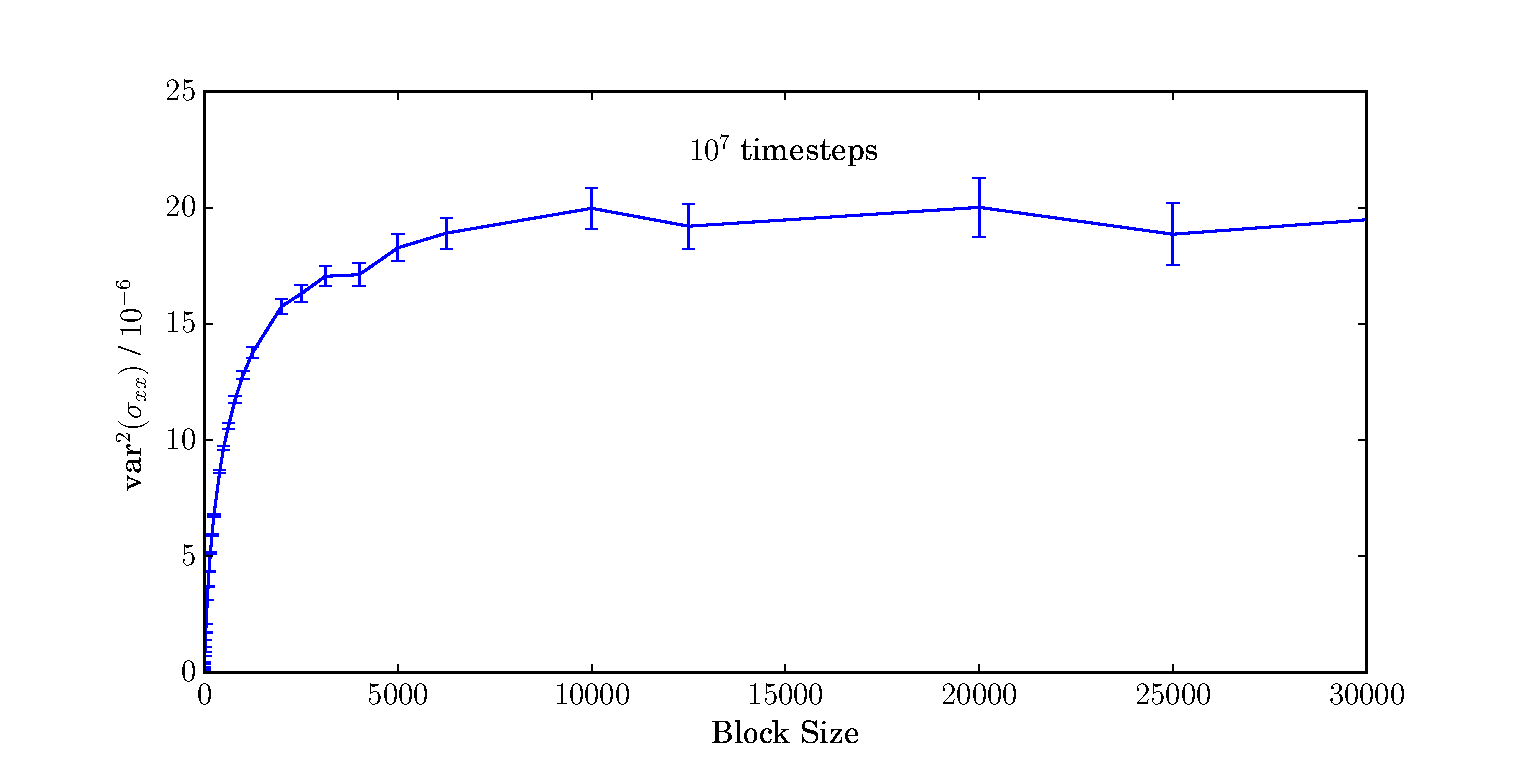
\includegraphics[scale=0.65]{block_average_10e6.eps}
	\\
        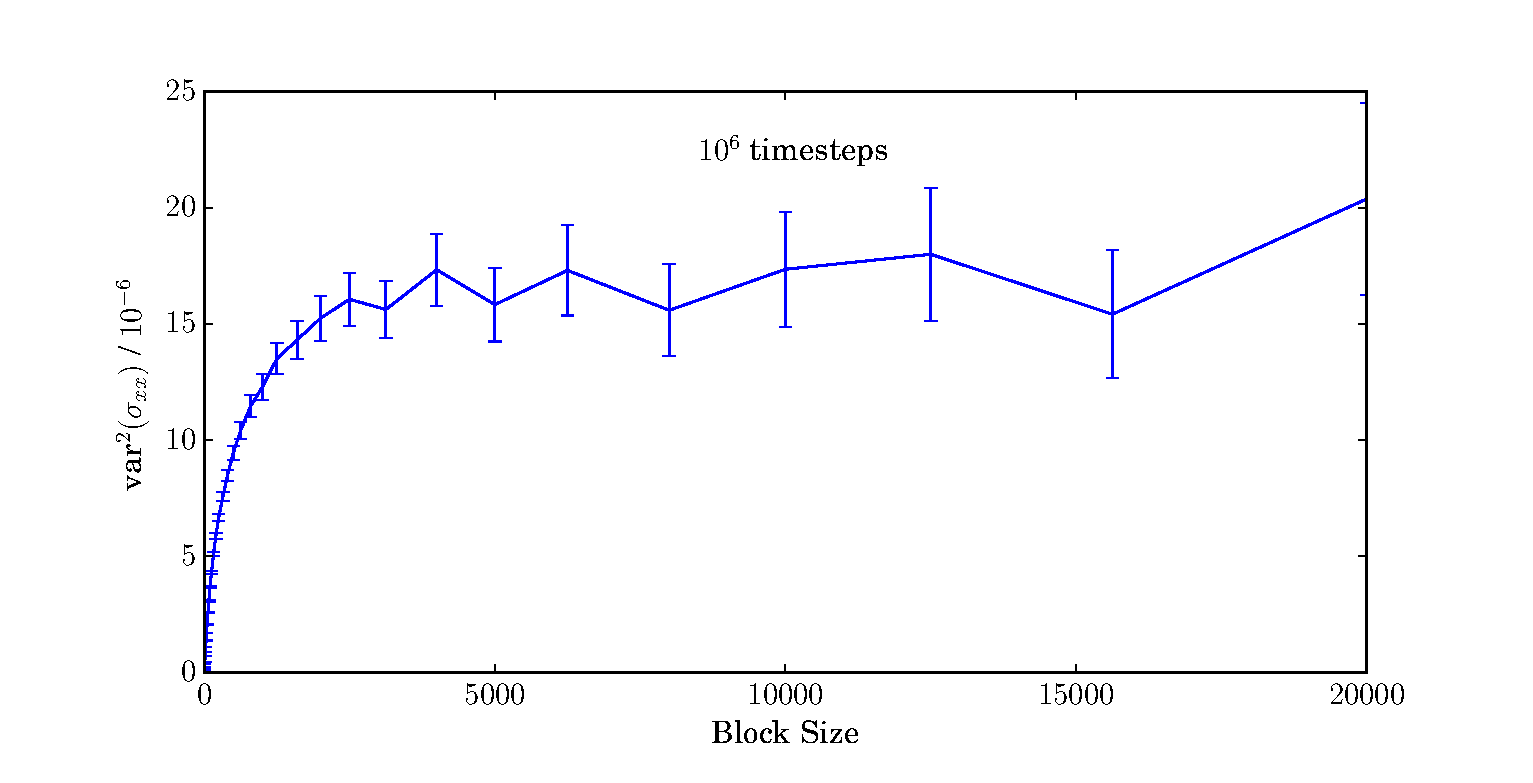
\includegraphics[scale=0.65]{block_average_1e6.eps}
	\caption{The blocking analysis for a simulation time of 10,000,000 timesteps and 1,000,000 timesteps shows clear plateaus in the estimate of the error at block sizes of 10,000 and 5,000 respectively.
This can be used to estimate the size of blocking needed to decorrelate data in the correspinding molecular dynamics simulations.}
\label{blocking}
\end{figure*}

Using a standard binary mixture simulation identical to those used to calculate the Marangoni forces at the interface, a blocking analysis was carried out for a simulation time of $10^{6}$ timesteps and $10^{7}$ timesteps as shown in Fig \ref{blocking}.
These data show a clear plateau at a block size of 10,000 timesteps for the longer simulation time and 5,000 timesteps for the shorter run, with little increase in the error of $\sigma^{2}$ until a much larger block size.
This information can be used to infer a suitable size for block averaging data within a LAMMPS simulation in order to yield sufficient decorrelation of individual samples and a good estimate of the statistical error. 

\section{Computational details}
All molecular dynamics simulations were carried out using the LAMMPS (Large Atomic and Molecular Massively Parallel Simulator) package.\cite{LAMMPS}
Additional processing was carried out using Numpy.\cite{NumPy}
All graphical figures were plotted using Matplotlib.\cite{MatPlotLib}

